\documentclass[11pt,journal]{IEEEtran}

\usepackage{times}
\usepackage{amssymb}
\usepackage{amsmath,amsfonts}
\usepackage{amsthm}
\usepackage{graphicx}

\usepackage{color}
\usepackage{xcolor}

\usepackage{scalefnt}

\usepackage{pgf}
\usepackage{tikz}
\usetikzlibrary{shapes.symbols,shapes.callouts,decorations,shapes.geometric,arrows}

\usepackage{hhline}
\usepackage{multirow}
\usepackage{array}
\usepackage{pdfpages}
\usepackage{subfigure}
\usepackage{algorithm}
\usepackage[noend]{algpseudocode}
\usepackage{balance}
\usepackage{epsfig}


\newcommand{\todo}[1]{} %essentially a block comment

\newtheorem{theorem}{Theorem}
\newtheorem{definition}{Definition}
\newtheorem{lemma}{Lemma}

\hyphenation{designs design algo-rithms devel-oped micro-pipeline after
  algo-rithm AFSM AFSMs}

\begin{document}

\title{Smart Chessboard}

\author{Nicole Sundberg, Griffin Rodgers, Kenan Ntambwe, Jack Marshall
  \thanks{The authors are in the Computer Engineering
    department at the University of Utah.}
}
\maketitle


\begin{abstract}
Chess is an incredibly fun game, but can often feel extremely intimidating to newcomers. With a variety of specialized pieces that each have their own movement scheme, learning and having fun with chess can feel like a lofty goal for those that have never played before. Furthermore, increasing your skill and understanding of chess can be difficult when games become complicated and difficult to recall. For these reasons, the Smart Chessboard was created.  The Smart Chessboard is a chessboard that teaches players how to play chess by clearly indicating possible moves when pieces are lifted.  The board also records moves alongside an application that tracks game statistics and more so that even seasoned chess players can retrospectively analyze their gameplay. The board will indicate possible moves via LEDs under the chess squares and will keep track of pieces lifted or moved. An application will also display the results and progress of the match per account. An AI algorithm will allow the player to play on the chessboard against a computer player so that learning can happen even without a chess partner. 
\end{abstract}

\section{Introduction}

\IEEEPARstart{C}{hess} is a world-known and widely enjoyed game. However, its complexity leaves many potential players struggling due to the many pieces, rules, and movement schemes. In an effort to create a fun and easy way to teach new chess players along with supplement the learning of more experienced players, the Smart Chessboard was created. 

This chessboard allows new and experienced chess players to benefit by showing possible moves and checking rules but also recording match history for virtual playback through the companion application. The Smart Chessboard shows players legal moves by lighting up the squares when pieces are lifted. The board also detects invalid or illegal moves and alerts the players with the board lights as well.  The chessboard will work alongside the companion application to record times and game history, allowing for clear growth and progress to be shown to players as they look through their previous games. The board also allows single-player mode where users can learn without the need of another physical chess player, allowing for easy learning at any time or place.

Using sensors and bluetooth connectivity, the board is able to determine when pieces are picked up or put down and record game data. Through algorithmic checking and the use of LED lights the board will also determine move legality and visualize legal moves when a piece is picked up.

%** \textbf{TODO: describe comparisons to other solutions, advantages to this one} **
There are programs designed to teach newcomers chess, but they do not often pair with a physical board. The creation of a physical board allows for more tactile learning styles and for users to learn in a more hands-on way that promotes a better understanding of the game overall. On top of this, these programs often do not allow for virtual replaying matches to determine mistakes or errors made or saving and tallying game statistics to show overall progress. Because of this, the Smart Chessboard is a more active and well rounded solution that is better able to engage the audience.


% Refer to figures as follows:
% The circuit in Fig.~\ref{fig:circuit}.

% Citations are as follows
% Algorithm returning longest netlist delay path \cite{knuth:book1973}.
%\subsection{Project Demonstration}
To demonstrate the Smart Chessboard, the physical custom chessboard along with the running companion app will be available to interested parties. When they lift a piece on the board, all valid moves and their associated squares will light up on the board, and once the piece is placed on a valid square, that move is logged by our app that is connected to the board. The player would also have the option of playing against a chess AI, and the opposite end of the board will indicate which pieces needed to be moved on behalf of the AI when the AI takes its move. The application will also have a co-demonstration where we can showcase the game history functionality and allow the user to play back previously played games.

\section{Background}



\subsection{Related Work}

Similar products to our chessboard design are on the market as both commercial products and open-source hobbyist projects. These products generally suffer from at least one of the following problems: high cost, requires access to specialized tools (e.g. 3D Printer), or lack quality of life features. Despite these shortcomings, many of them contain other novel features, such as move assistance, where you can enable and configure the board to suggest optimal moves in the current game, or multi-colored LED indicators to indicate the strength of a move. We have found two examples of smart chessboards, one from the consumer space and the other from academia, and will provide a short explanation of their functionality as well as our criticisms with each design.

% You may want to subsection the background.

% Include plenty of figures.

%% This is a figure with two side by side images.
% \begin{figure}[thb]\centering
%   \begin{minipage}{0.48\columnwidth}
%     \centerline{\psfig{file=images/IMG_2712-crop.jpg, height=30mm, angle=0}}
%     \begin{center} (a) \end{center}
%   \end{minipage}
%   \begin{minipage}{0.5\columnwidth}
%     \centerline{\psfig{file=images/img2.png, height=30mm, angle=0}}
%     \begin{center} (b) \end{center}
%   \end{minipage}
%   \caption{The die and substrate (a), and complete system (b).}
%   \label{fig:chip-system}
% \end{figure}

% This is how you label a section of the text:
% \label{sec:falsePath}
ChessUp is a smart chessboard that was funded via Kickstarter. Some of its features include LEDs to signal correct/incorrect moves, a companion app allowing play against friends and family, and unique ''touchsense pieces'' that can detect when a piece is touched and show the available moves for that piece \cite{chessup}. In our research of the ChessUp, we noticed that to access some basic features, such as the chess clock, requires a smart phone with the ChessUp app installed and placed next to the board and left there for the entire game. We also noticed reviews stating that the app connectivity is finicky, with apparent disconnects from online games as well as no indication of when the opposing online player has resigned from the game, other than ceasing to make moves.

Assistive Chessboard is a project proposal from a group of electrical engineering students at the University of Illinois in Fall 2017. This project proposal details an assistive chessboard project that is very similar to the one proposed here. However, this proposal only details the hardware implementation of the board, and does not cover any software components at all other than a passing mention of a mobile app that communicates with the board via Bluetooth. The Assistive Chessboard implements features such as entirely wireless play, with the integration of the previously mentioned Bluetooth and a rechargeable battery, enabling a wireless playtime of up to 4 hours. It uses hall-effect sensors under each square of the chessboard to detect if a piece is placed on any given square. In addition, it also uses multi-colored LEDs to signal to the player whether a move is correct or incorrect. It also integrates a basic LCD display and various buttons for user interactivity, however the details are scant on how these were to be implemented. One novel feature here is the use of a 24-bit shift register to select and manipulate the color of the integrated LEDs. The authors also designed custom PCBs for each of the squares of the board containing the LED and sensor circuits \cite{assistivechess}. We believe that this is a good approach for prototyping as it allows for fast diagnosis and swapping of PCBs if a fault is detected, however this does make wiring and overall organization of the board more complicated.
% You can include equations such as Eqn.~\ref{eqn:booleanDifference}
% \cite{boole:book1872}.

% \begin{equation}
%   \frac{df}{df_x} = f_x \oplus f_{\overline{x}}
%   \label{eqn:booleanDifference}
% \end{equation}



\section{Implementation}
\subsection{Hardware}
The hardware design for a chessboard required more thought and testing than we initially expected; however, it ended up taking less of our time than the software components and physical assembly of the chessboard. Our design philosophy for this project was centered primarily on cost, with us wanting our chessboard to be much lower cost than some of the commercially available alternatives. Our focus on cost influenced many decisions, including the selection of the Raspberry Pi Pico W as our microcontroller. This affordable option (around \$10) provides both Bluetooth and WiFi capabilities, essential for our design. For cost reasons, we also chose to power every component of our design with 5V, because 5V power supplies can be found for very low cost and also allow the entire circuit to be powered via USB. The following sections detail the design process and decisions for key hardware components.
\subsubsection{Sensing Circuit}
The key aspect of the hardware implementation for the chessboard is the sensing circuit that can detect whether a chess piece is located on a specific square of the board or not. To accomplish this task, we used the Texas Instruments DRV5053 Analog-Bipolar Hall Effect Sensor. This sensor outputs a steady voltage ranging from 0V to 2V, with a 1V output when no magnetic field is detected. The voltage drops below 1V when it detects a magnet's negative pole and rises above 1V when it detects a magnet's positive pole. Therefore, each chess piece has an embedded magnet, with the positive pole facing outward for white pieces and the negative pole facing outward for black pieces. The magnitude of the rise or drop corresponds to the strength of the magnetic field applied to the sensor. With this in mind, we prototyped this basic sensor on a breadboard in May 2024 and discovered that this sensor serves our purposes well. Please see Figure \ref{sensorcircuit} for the circuit diagram of the DRV5053 recommended in the data sheet that we used in both prototyping and final assembly.
\begin{figure}[ht]
  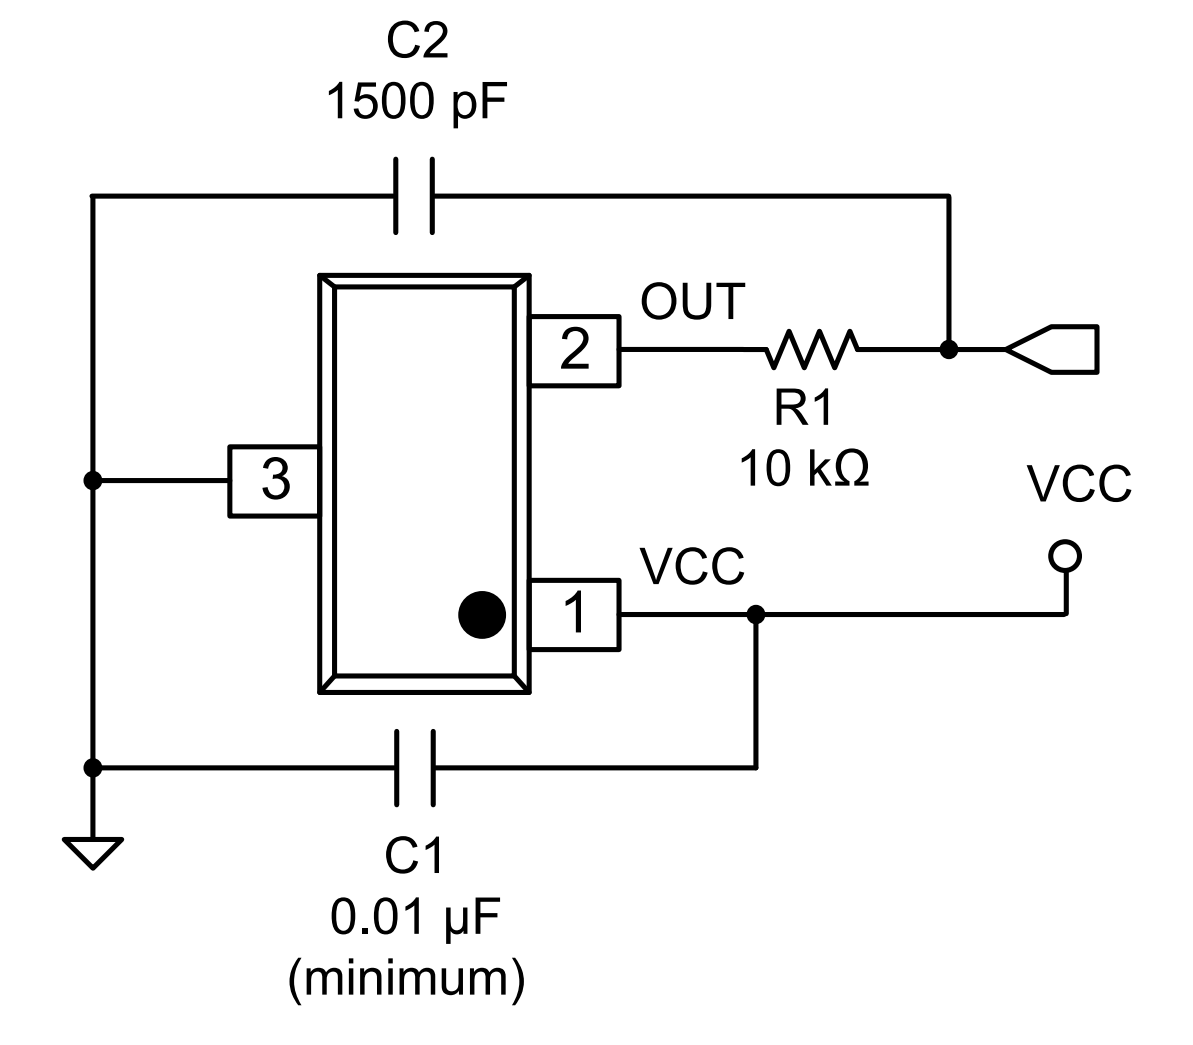
\includegraphics[width=\linewidth]{SensorCircuit.png}
  \caption{Sensor Circuit Diagram}
  \label{sensorcircuit}
\end{figure}
The challenge was that we needed to have 64 individual sensors for our chessboard, so that each space on the board could detect the presence of a chess piece. Our selected micro-controller, the Raspberry Pi Pico W, did not have enough analog to digital converter (ADC) channels nor enough GPIO pins to support 64 inputs from our analog sensors, so we had to find another solution. We prototyped a few different solutions, one using external GPIO expander chips that communicated with the Pi Pico via SPI, and another utilizing external 8-channel ADC chips that also communicated via SPI. We chose the MCP3008 8-bit ADC from Microchip, as using a dedicated ADC for each space allowed us more flexibility in software to set things such as the sensitivity of the Hall-effect sensors in detecting the chess pieces. Had we gone with a GPIO expander chip, we would have had to use external circuitry to set this sensitivity. Confirming the functionality of this chip in combination with the sensor circuit was relatively easy, as all we had to do was connect the MCP3008 to one of the SPI buses on the Pi Pico, and then connect the output of each sensor to one of the 8 inputs on the ADC. We needed 8 MCP3008 chips to support 64 sensors, and all 8 of the MCP3008 chips were hooked up to a single SPI bus on the Pico, limiting the number of GPIO pins required for this approach.
\subsubsection{Integrated PCB Design}
Once we confirmed that the prototyped piece sensing circuit would fit our needs and that we could read all of them via our external ADCs, we moved onto designing a PCB around these components for a more streamlined product. We used Autodesk Fusion to design the PCB as it is graciously provided to University of Utah students at no cost. We decided we wanted a modular approach to the PCB design, as designing a single PCB for an entire 64 space chessboard would not only be costly, but if a single sensor failed, the entire PCB would need to be replaced. So we decided to split the PCB in 8 pieces, each one corresponding to an 8 square row of the chessboard. We also decided that each square on the board would be 1 inch by 1 inch, to keep it compact. With these requirements in mind, we designed the PCB shown in Figures \ref{pcbschematic}-\ref{pcbdesign}. The dimensions of this PCB are 1 inch by 8.5 inches. There was also a small outline made in the silkscreen next to each sensor to accommodate the placement of LEDS and two screw holes left in each board for mounting purposes. The extra half inch on the end is to accommodate the presence of the MCP3008 as well as header pins for the connections to the Pi Pico and to external power and ground. This design was then sent to OSHPark for production, and 9 total were ordered, as OSHPark requires you to order prototype PCBs in batches of 3. 8 of them were then hand soldered and functionality was confirmed with the first revision.
\begin{figure}[ht]
  \includegraphics[width=\linewidth]{PCBSchematic.png}
  \caption{PCB Circuit Schematic}
  \label{pcbschematic}
\end{figure}
\begin{figure}[ht]
  \includegraphics[width=\linewidth]{PCBLayout.png}
  \caption{PCB Design}
  \label{pcbdesign}
\end{figure}
\subsubsection{LEDs}
\subsubsection{Assembled Prototype}
With all the components in hand and all 8 PCBs soldered and validated, we were ready to begin designing and assembling the chessboard itself. We created a 3D model of a chessboard that would house all of our physical components in Autodesk Maya and printed it using transparent PETG filament on a 3D printer. The housing was too big for the print area of the 3D printers available to us, so we had to print it in two parts and glue them together. We printed two total revisions of our housing, and the second revision only needed an extra hole added for wiring purposes. Once we printed the housing, we inserted the eight PCBs and adhered them to the board using mounting putty, which we used because the top layer of the chessboard was not thick enough for us to use the screw holes for mounting the PCBs. We then inserted a breadboard containing the Pi Pico, as well as the buttons and display, and wired it all together using standard breadboard jumper cables. For the chess pieces, we found a free model and modified it to have a hole in the base, and glued a magnet in each piece. Please, see Figures \ref{boardtop}-\ref{boardbottom} for pictures of the final assembled prototype.
\begin{figure}[ht]
  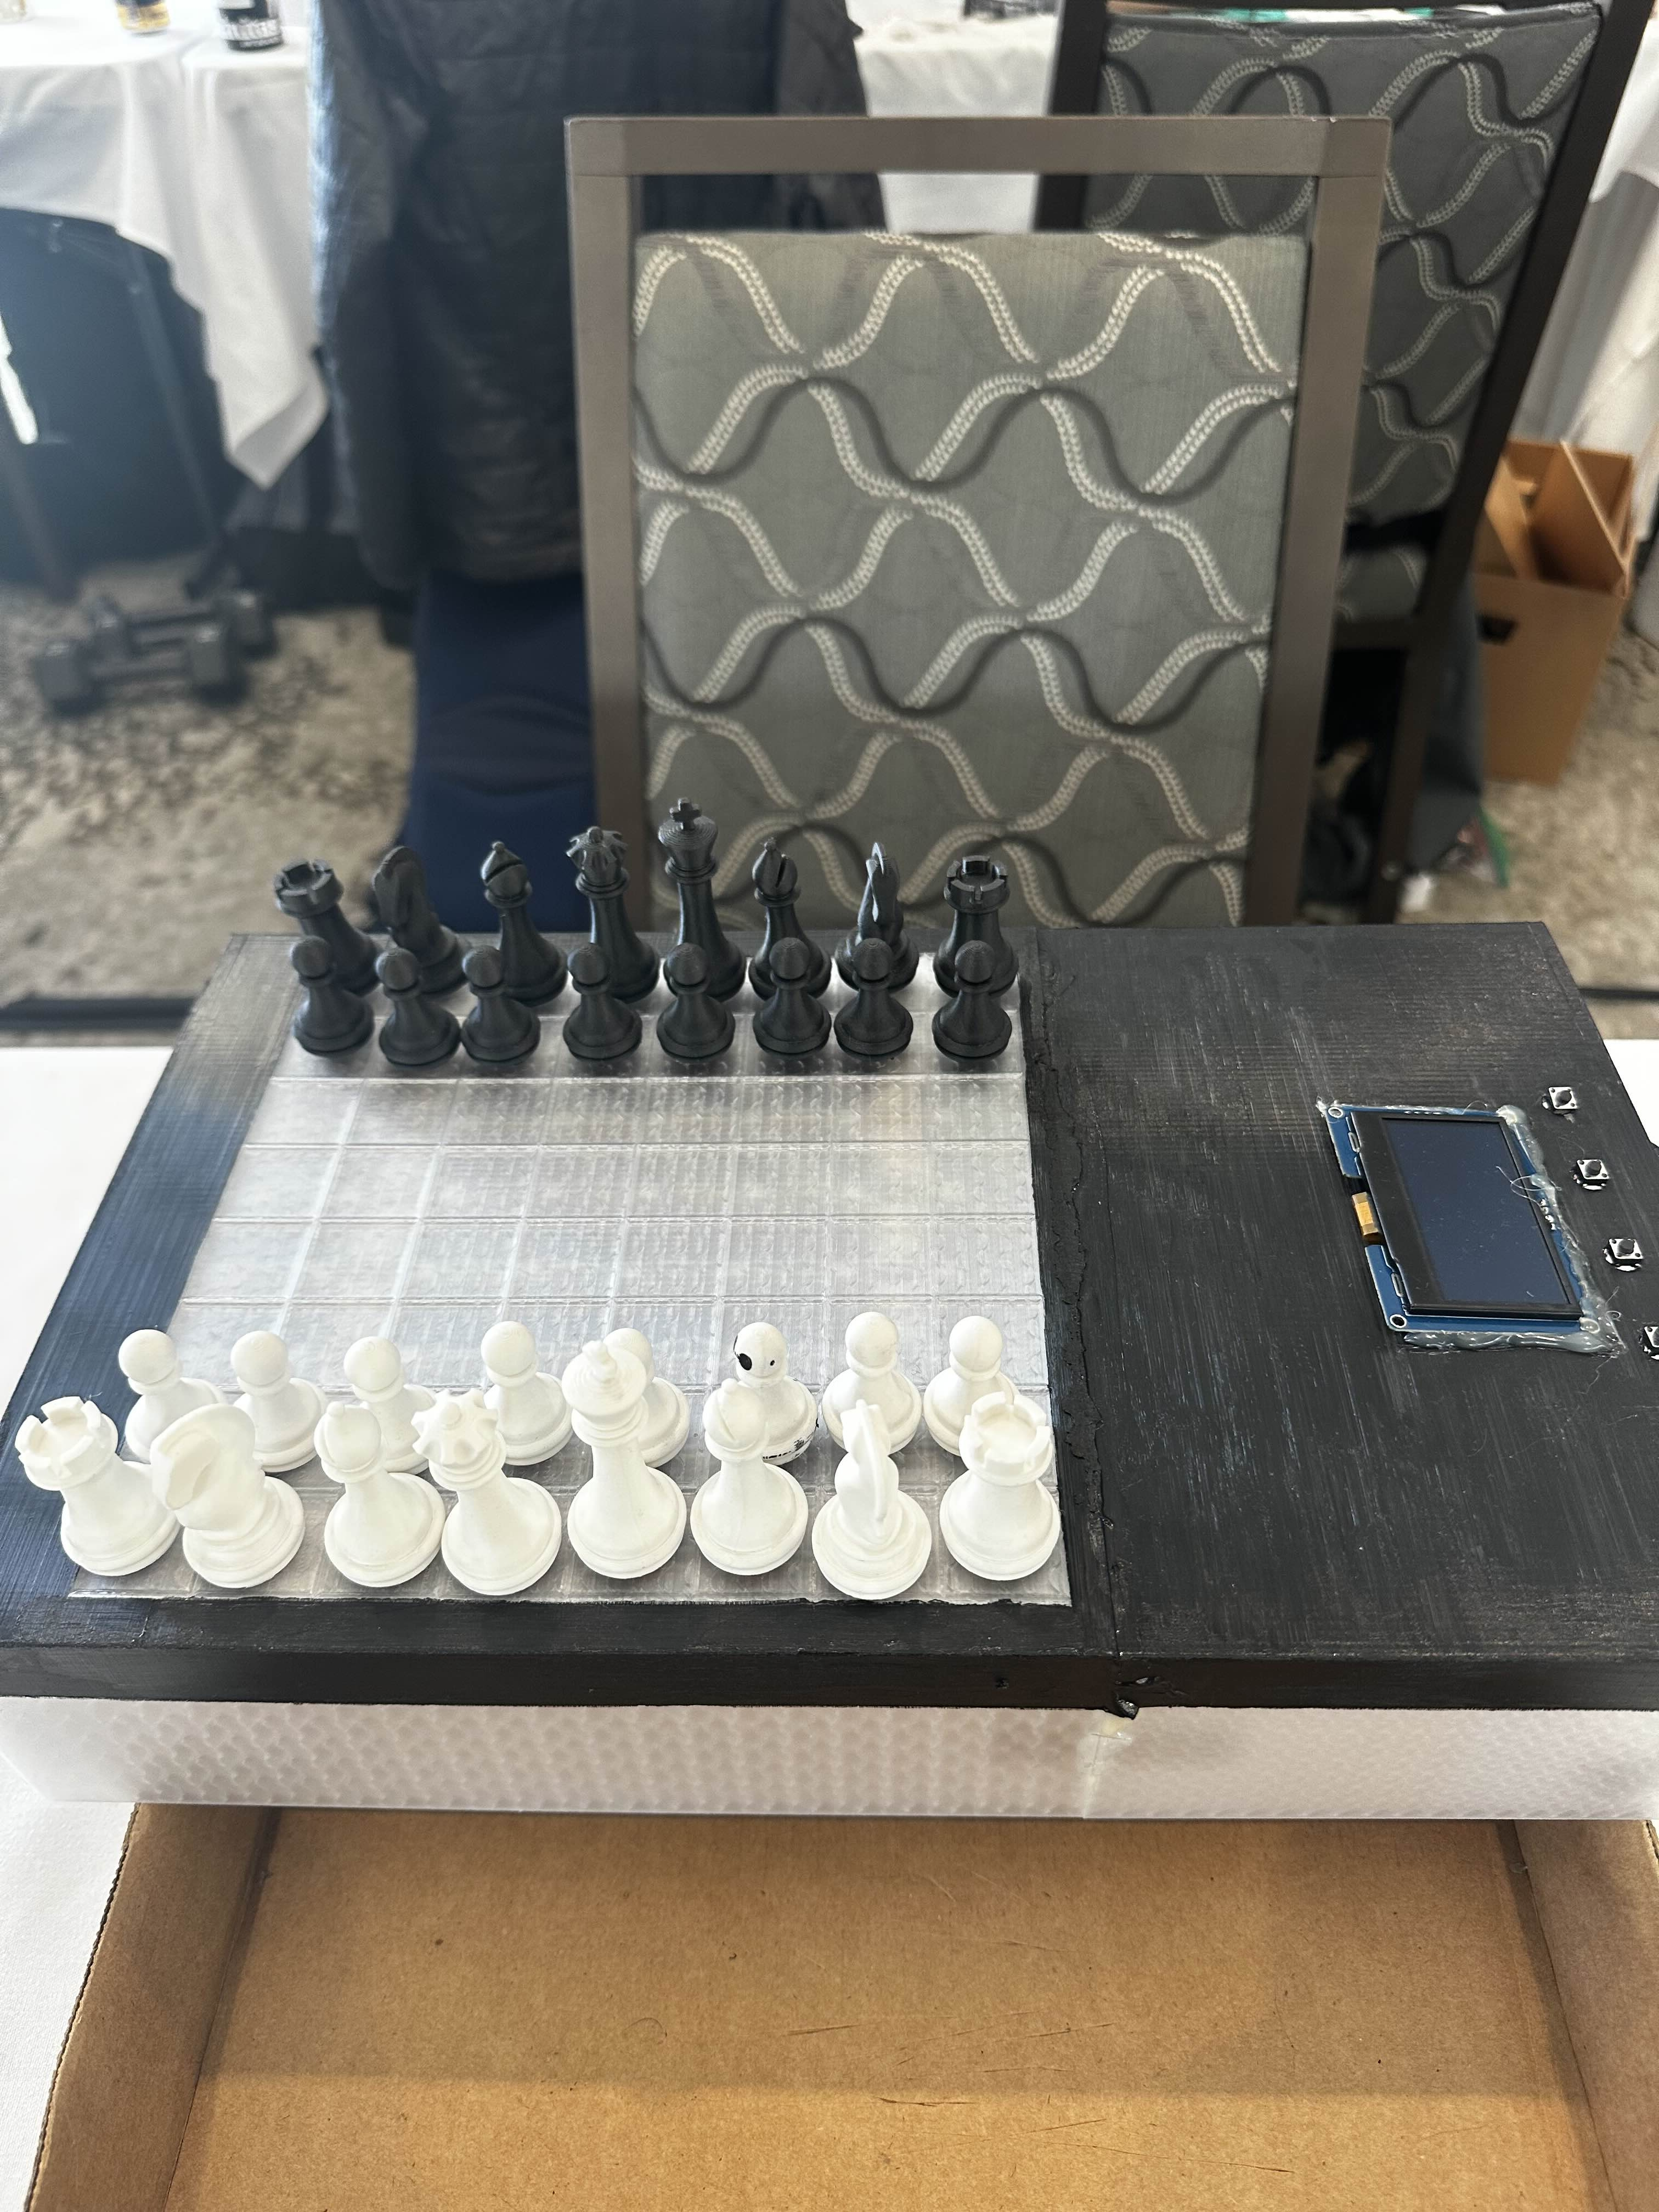
\includegraphics[width=\linewidth]{boardTop.jpg}
  \caption{Top view of assembled chessboard}
  \label{boardtop}
\end{figure}
\begin{figure}[ht]
  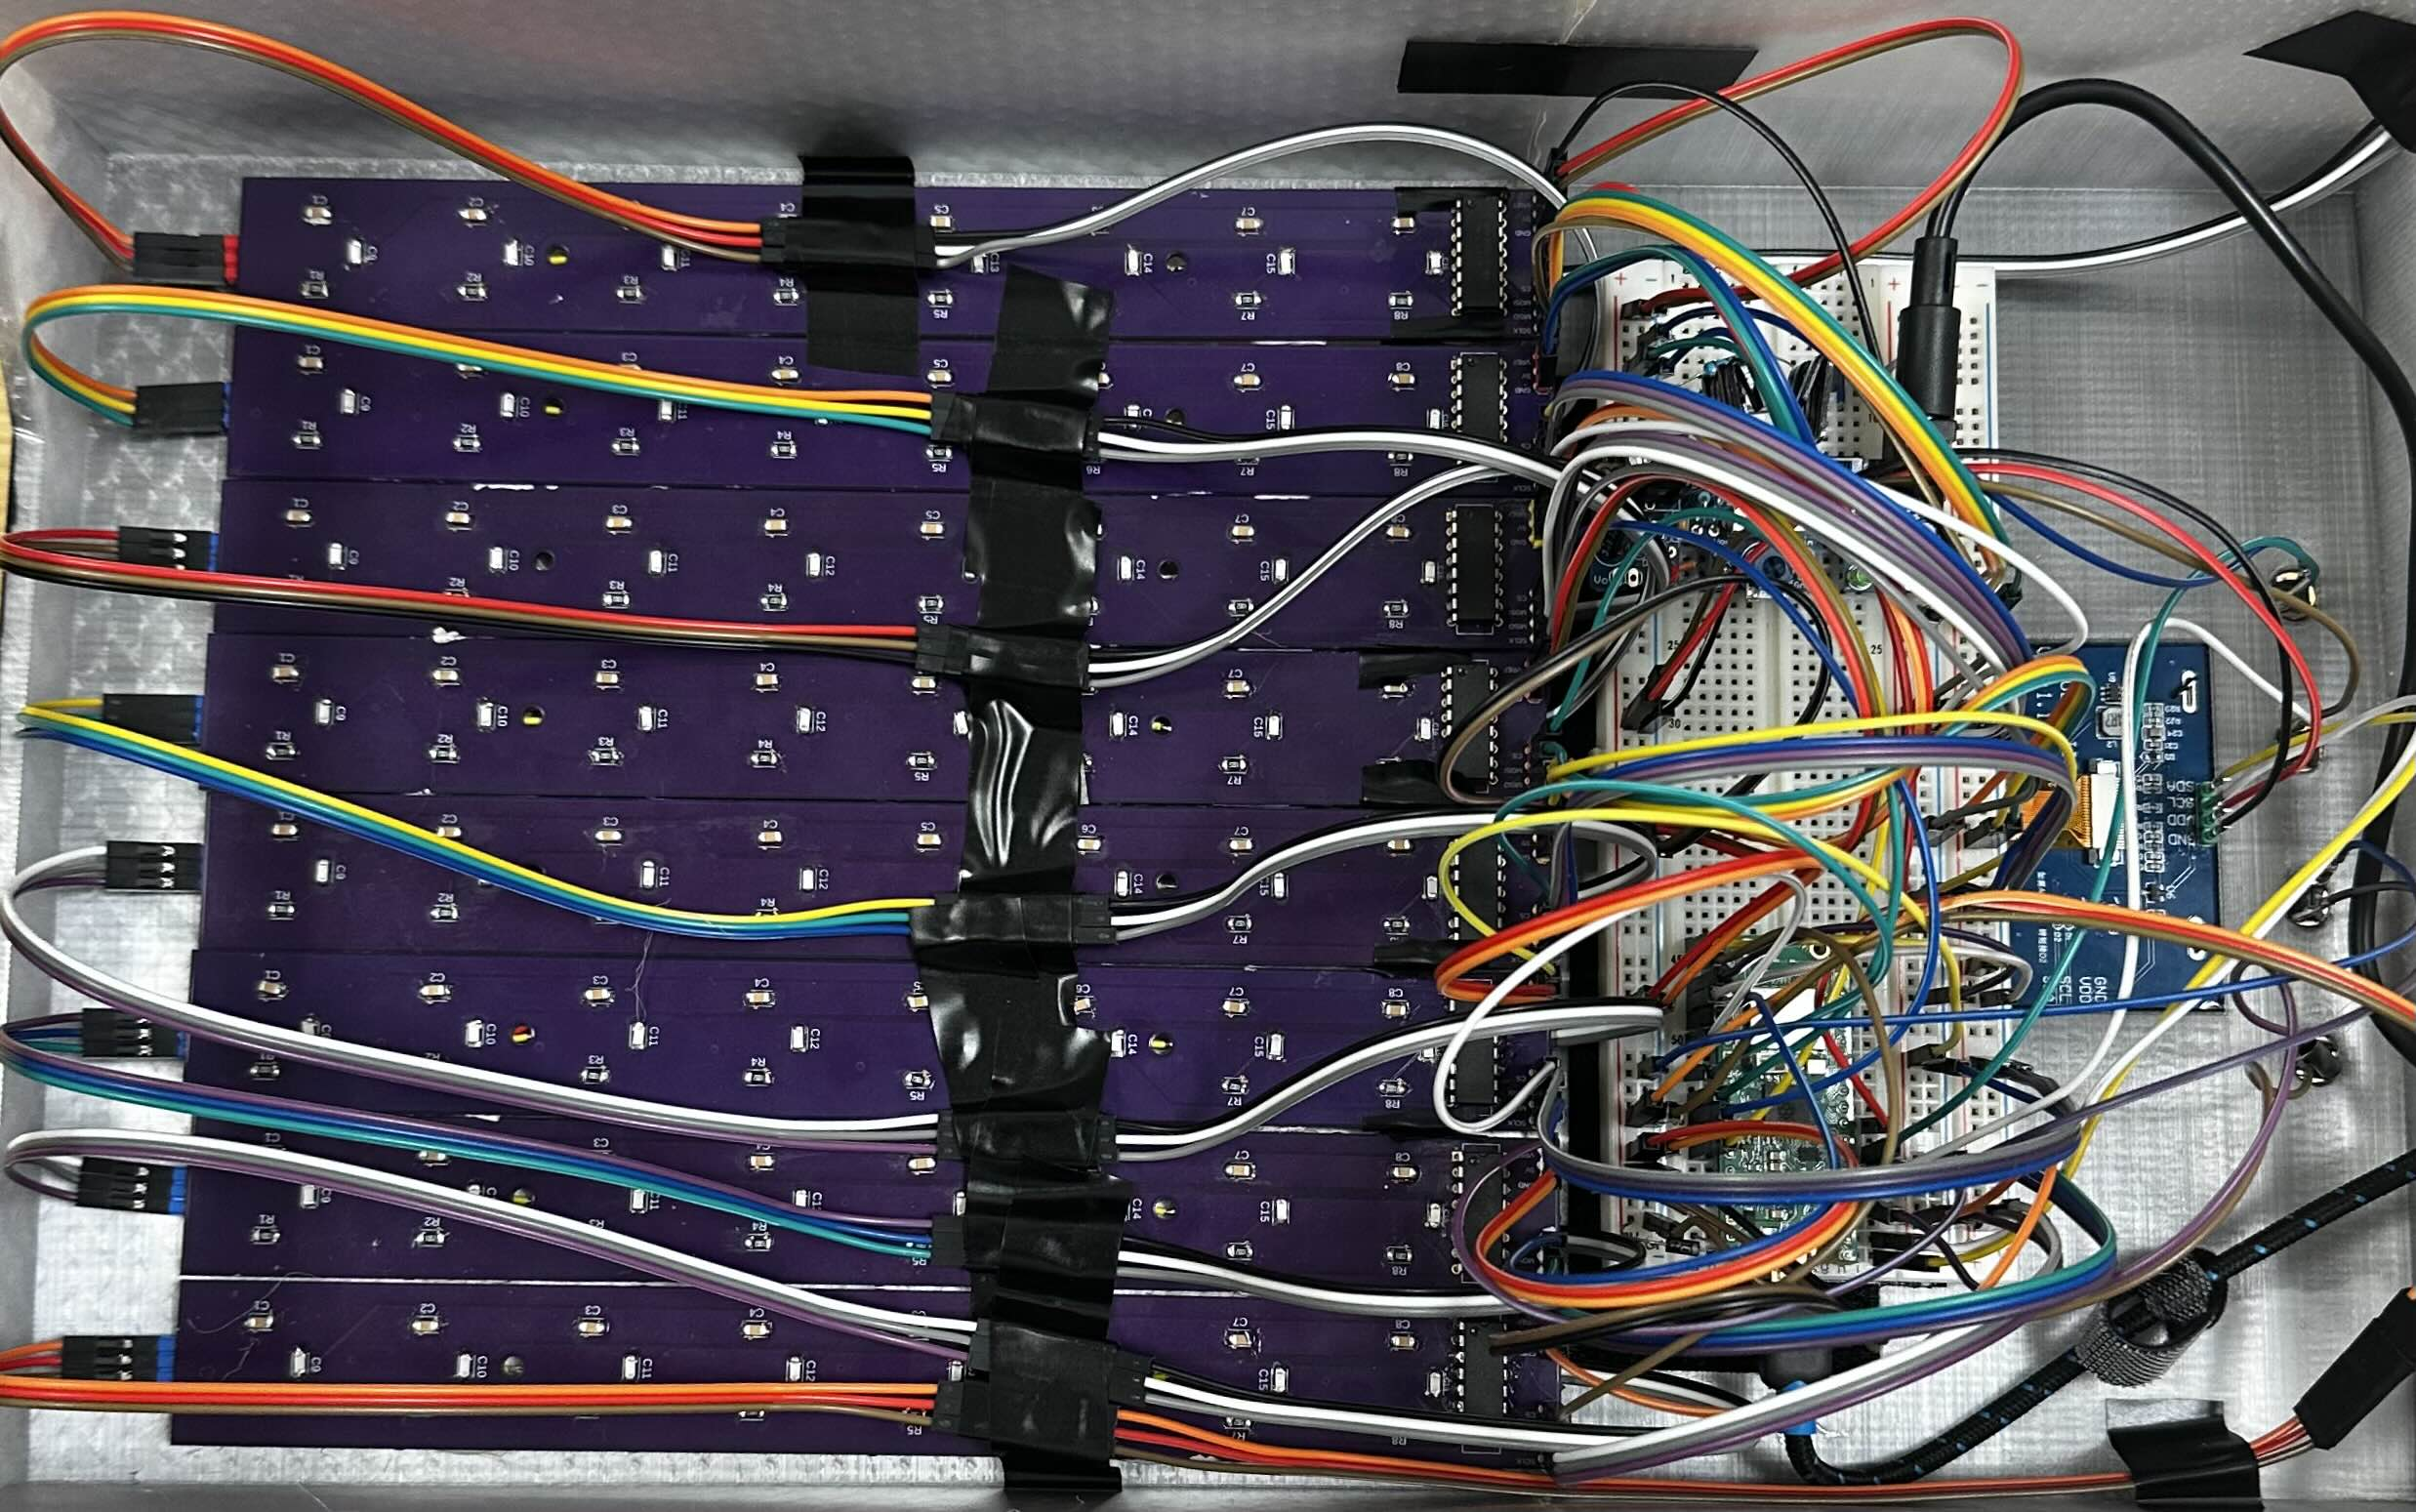
\includegraphics[width=\linewidth]{boardBottom.jpg}
  \caption{Bottom view of assembled chessboard}
  \label{boardbottom}
\end{figure}
\subsubsection{Bill Of Materials}
The Smart Chessboard needs a physical, custom made body in addition to several hardware components. The following lists the materials used. The components will be listed in the order of quantity, part description, vendor, and unit price. Refer to Table \ref{bomtable}.
\begin{center}
\begin{table}[ht]
\caption{Bill of Materials}
\begin{tabular}{|l|l|l|}
\hline
\textbf{Qty} & \textbf{Part}                        & \textbf{Source} \\ \hline
1            & Roll of LEDs                         & Amazon          \\ \hline
64           & DRV5053 Hall-effect sensor           & DigiKey         \\ \hline
80           & 1 $\mu$F 1206 SMD Ceramic Capacitor  & DigiKey         \\ \hline
64           & 1 pF 1206 Ceramic Capacitor          & DigiKey         \\ \hline
64           & 10 k$\Omega$ 1206 SMD Resitor        & DigiKey         \\ \hline
1            & 1kg Transparent PETG Filament        & Amazon          \\ \hline
1            & Raspberry Pi Pico WH                 & PiShop.us       \\ \hline
32           & 15mm x 5mm Flexible hobby magnet     & Amazon          \\ \hline
8            & Microchip MC3008 ADC                 & Adafruit        \\ \hline
1            & Power Delivery board                 & Amazon          \\ \hline
4            & Push button                          & Stock room      \\ \hline
1            & OLED I2C Display                     & Amazon          \\ \hline
\end{tabular}
\label{bomtable}
\end{table}
\end{center}
\subsection{Software}
\subsubsection{MicroPython Firmware}
Jack will contribute here
\subsubsection{Android App}
\subsubsection{Communication Protocols}
Jack will contribute here

% You probably want subsections for tasks, testing and integration,
% management and communication, schedule and milestones, risk
% assessment, bill of materials (not necessarily in this order)


% \section{Results}
% \label{sec:results}
% 
% This section probably won't be in the proposal.


\section{Conclusion}



\section*{Acknowledgment}

The authors would like to thank Romilly Cocking on GitHub for their MCP3008 MicroPython library. We would've had to spend a considerable amount of time writing a library ourselves and going over the documentation for the MCP3008 were it not for their work.\cite{cocking_pico_code_2023}



\bibliographystyle{IEEEtran}  % IEEEtran -- needs IEEEtran.bst
% Balance the citations to equalize the columns manually
% \balance
\bibliography{proposal}

\end{document}


% LocalWords:  Eqn df
